
\chapter{Literature Review}
\label{chap:chapter2}
Anomaly detection covers numerous things in cloud computing from security perspective. In order to understand them, the underlying concepts that might identify the source of vulnerabilities and threats must be understood. This section analyses those concepts, starting with an explanation on virtualization elements and then on multi-tenancy. Cloud services are also discussed, followed by the discussion of the concept of service providing in cloud  and the section ends with a discussion on anomaly detection.
\begin{figure}
    \centering
    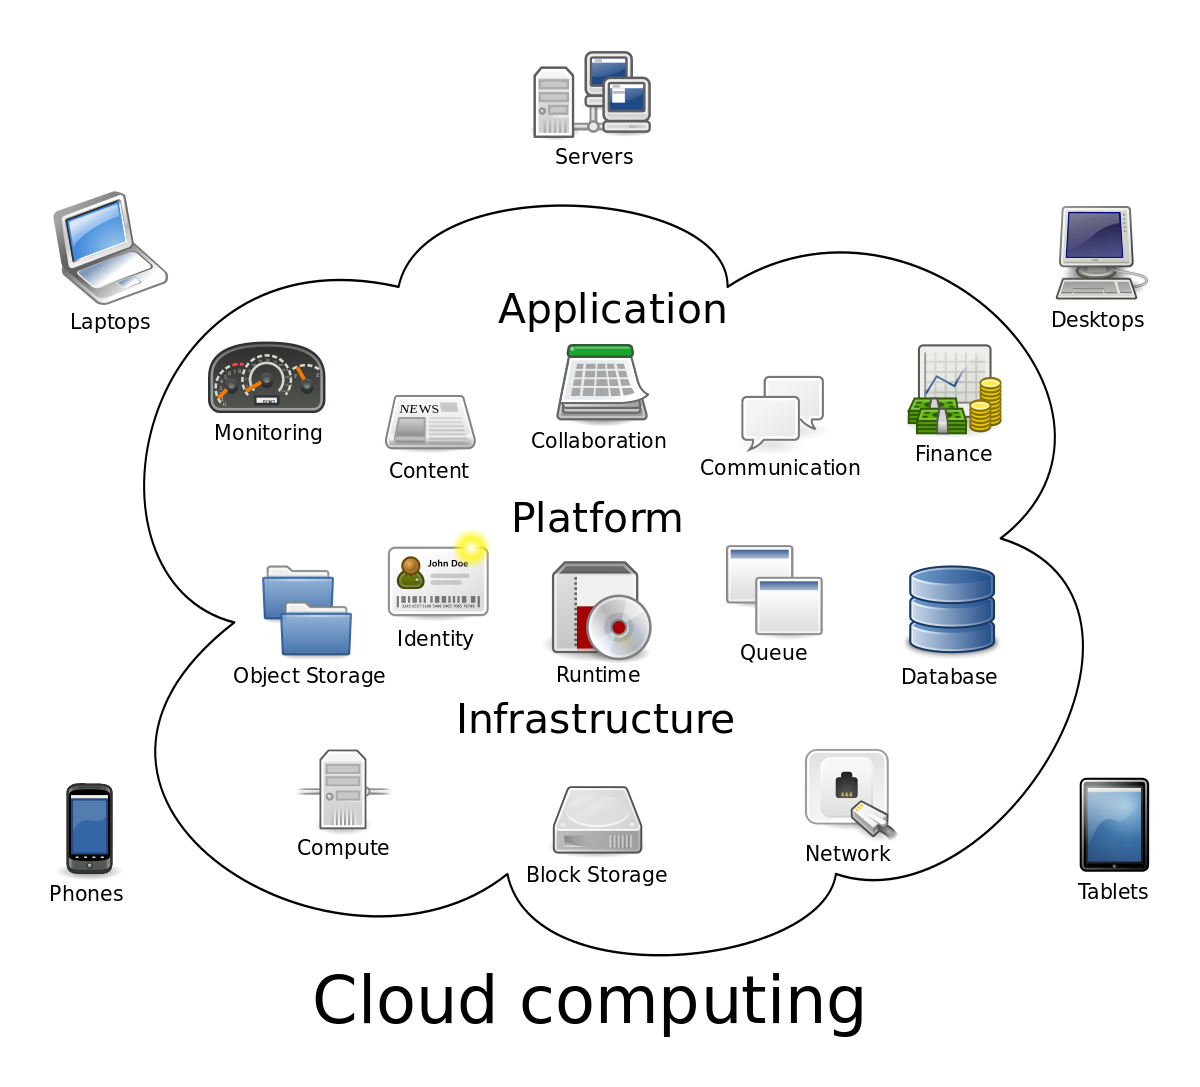
\includegraphics[width=10cm]{texfiles/images/Cloud_computing.png}
    \caption{Cloud Computing\cite{cloud33}}
    \label{fig:my_label}
\end{figure}
%    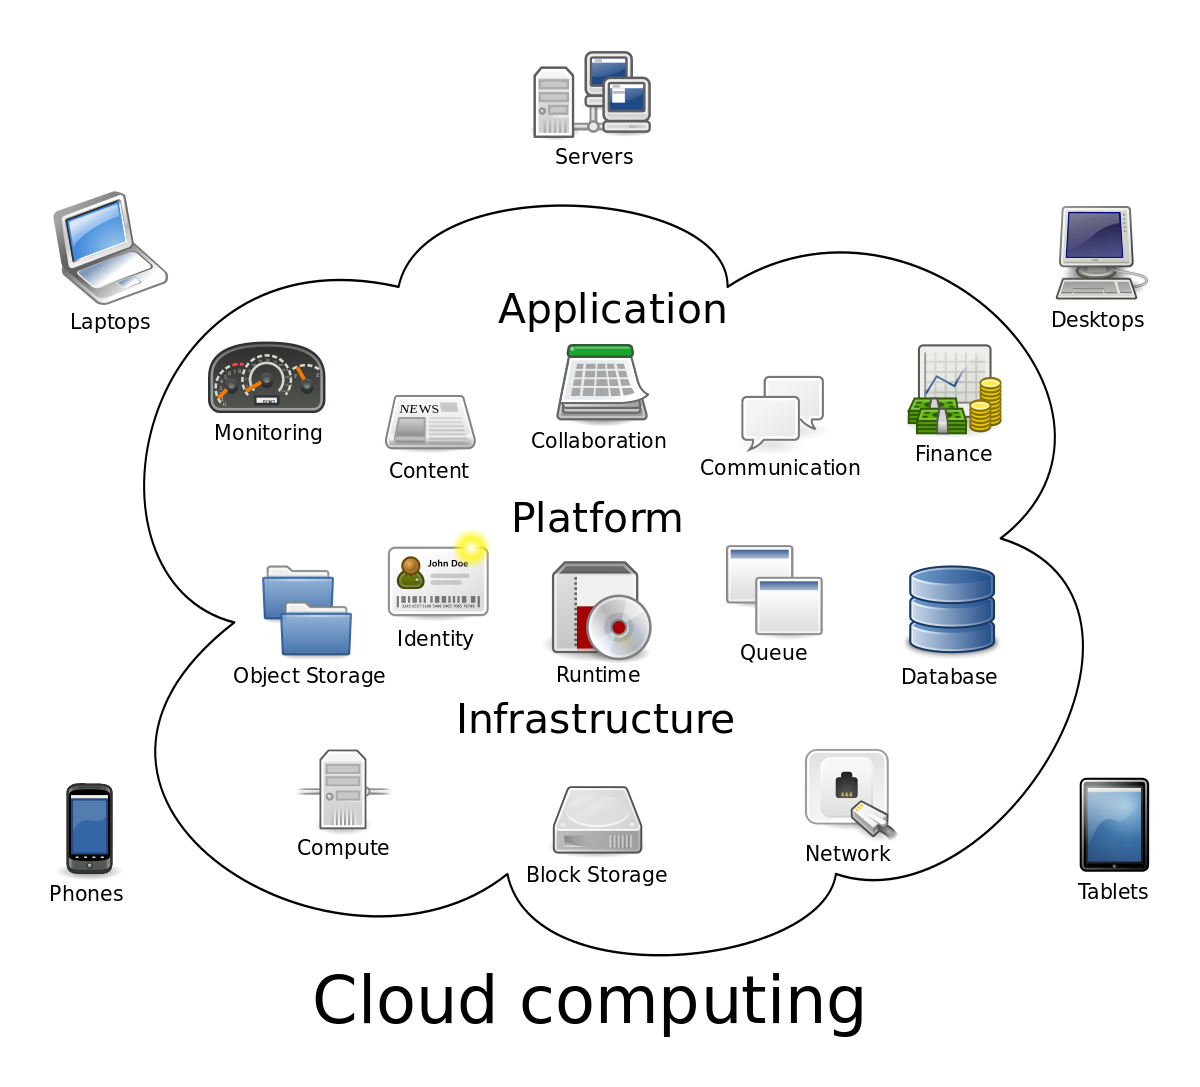
\includegraphics[width=10cm]{texfiles/images/Cloud_computing.png}
 %   \label{fig:cloud_computing_demo}
\newline
Four main models used for deployment of Cloud Computing are as follows \cite{mell62011}:\\
\textbf{Private Cloud:}  It is set up by a single organization for its own use or for customers.\\
\textbf{Community Cloud:} The infrastructure is provided for use by organizations which can have \\multiple customers.\\
\textbf{Public Cloud:} In this kind of deployment model general public is given access to resources in cloud on internet.\\
\textbf{Hybrid Cloud:} A hybrid cloud is a computing environment that combines a public cloud and a private cloud by allowing data and applications to be shared between them.\\
Security Issues with respect to Cloud Computing \cite{fernandes2014security} have been widely discussed both in academics and industry several international conferences have focused on this subject :\\
Confidentiality\\
Virtualization Level Issues\\
Multi Tenancy Issues\\
VM Isolation Issues\\
Virtual Network Issues\\
Virtual Machine Introspection Issues\\
VM Management Issues\\
Application Level Issues\\
Isolation Issues\\
Synchronization Mechanism Issues\\
Data Storage Level Issues\\
Outsourcing Issues\\
Data Deletion Issues\\
Network Level Issues \\
\newline
DoS attacks, and DDOS attacks affect cloud computing infrastructure and services. These type of attacks are major attacks which affect the available services. The Cloud Infrastructure \\provided by vendor could be a victim of such attacks but apart from that it could also be participating in such attacks. Botnets , botClouds can be deployed in Cloud Environment \cite{de2019cyber} to launch such attacks. Hence from security perspective it is important to identify such an issue that may exist in underlying cloud infrastructure.\\
Three main type of service models used in Cloud Computing are as following :\\
Infrastructure as a Service (IaaS)\\
Platform as a Service (PaaS)\\
Software as a Service (SaaS)\\
In \cite{linthicum2017connecting} author discusses that with the advent of cloud computing a lot of data has been generated how this data has been impacting the world and there is a lot of growth in the data of devices that have been connected. So, with the improvements in bandwidth and availability. In the context of the Internet of Things, the trouble with the cloud is that data needs to be sent back from the sensors gathering info, such as a Nest thermostat or a Fitbit wristband, to a database in a remote public cloud. The time that it takes for the data to be transferred from the device or sensor to the remote public cloud, that is the latency, is often too great to meet the requirements of the IoT system. The cloud complicates this process even more.We’re focused on centralized computing, thus there will be latency. Now, instead of sending the data back to the data centre on the other side of the factory, we send it to a remote cloud server that can be thousands of miles away. To make things worse, we send it over the open Internet.\\
In \cite{shen2017block} discussion about data sharing has been made. As how participants must share data. Protocols have played an important role. Protocols have played an important role in transfer of data in case of cloud computing. Storage has become a hot topic in today’s cloud computing world. We prefer to store all types of data in cloud servers, which is also a good option for companies and organizations to avoid the overhead of deploying and maintaining equipment when data are stored locally. In cryptography, a key agreement protocol is a protocol in which two or more parties can agree on a key in such a way that both influence the outcome.  This kind of protocol has widespread application in technology of internet and cloud computing.\\
In \cite{shirazi2017extended} mobile edge computing and emerging models in fog computing have been discussed. Relation between them is evident. The approach in the paper is to examine and underpin the models that are existing in cloud computing. Characteristics of cloud like support of ubiquitous connectivity, elasticity, scalable resources and ease of deployment have played an important role in development of existing cloud computing infrastructure. Research community has proposed new technologies namely fog and cloud. These technologies have been labelled in the paper as extended cloud they allow computing needs to be performed closer to source of data. This results in improvement in quality of services provided since this results in reduction of delay in conveying data between end nodes and cloud. Such technologies have enabled support for new application and services example Google now, foursquare and both are location aware applications for mobile platforms. Further this can be extended to services like autonomous vehicles robotics, public safety and augmented reality.

The acceptable level of service depends upon user expectations. Now these days users require rapid access to service like always on always available. So a new term has popped up known as resilience \cite{shirazi2017extended}. Resilience is concerned with availability of services and maintaining confidentiality and integrity of information in face of challenges. Resilience has become a fundamental property of cloud service provisioning platforms. With the advancement in wireless related technologies security and resiliency have become key issues when considering Mobile Edge Computing Services. With regards to edge model there are few threats also which have evolved. For example, infrastructure related threats, virtualization related threats, privacy related threats.
Fog computing model was originally conceived by Cisco as an extension of cloud. The term fog was originally coined by Cisco as there is need to enable a platform that can cope up with the requirements posed by challenges put forward by Internet of Things. Another requirement in fog computing is privacy of data. In the paper detection and resilience mechanism have been discussed. 
The area that has been challenging to researchers is anomaly detection.
In September 2016 \cite{kolias2017ddos} website of computer security consultant Brian Krebs was hit with 620 Gbps traffic. At the same time a bigger DDoS attack using Mirai malware was done on French web hosting and cloud service provider OVH. Mirai’s source code was release by its creator soon after wards. Hackers offered Mirai’s botnets for rent with as many as 400,000 connected devices. More attacks happened in October 2016 using Mirai they took down hundreds of websites like Twitter,Netflix,Reddit, Github for several hours. Mirai spreads by infecting devices as web cams,DVRs, routers, then it finds out administrative controls of those devices by a brute force attack which relies on a dictionary of potential usernames and passwords.





